% !TEX encoding = UTF-8 Unicode
% !TEX TS-program = xelatex
% !TEX root = main.tex

\documentclass[xetex]{beamer}

%%%%%%%%%%%%%%%%%%%%%%%%%%%%%%%%%%%%%%%%%%%%%%%%%%%%%%%%%%%%%%%%%%%%
% Beamer settings

\mode<presentation>
{
  %\usetheme{Frankfurt}
  \useoutertheme[subsection=false]{smoothbars}
  \setbeamercovered{transparent}
  \setbeamertemplate{navigation symbols}{} %remove navigation symbols
  \setbeamercovered{invisible} %No transparent layers
}


\usepackage[many]{tcolorbox}
%\usepackage{tcolorbox}
\tcbuselibrary{skins,xparse}


\newcounter{ct}
\newcounter{contribution}

% put color to \boxed math command
\newcommand*{\boxcolor}{orange}
\makeatletter
\renewcommand{\boxed}[1]{\textcolor{\boxcolor}{%
\tikz[baseline={([yshift=-1ex]current bounding box.center)}] \node [rectangle, minimum width=1ex,rounded corners,draw] {\normalcolor\m@th$\displaystyle#1$};}}
 \makeatother
 \newcommand{\tboxed}[1]{\textcolor{\boxcolor}{%
\tikz[baseline={([yshift=-1ex]current bounding box.center)}] \node [rectangle, minimum width=1ex,rounded corners,draw] {\normalcolor#1};}}
 \makeatother

\usepackage{etoolbox}

\newtoggle{presentation}
\toggletrue{presentation}
%\togglefalse{presentation}

\newtoggle{euler}
\toggletrue{euler}
%\togglefalse{presentation}
 

% Loads configuration file

\input{./cfg/settings.tex}
\input{./cfg/fonts.tex}
\input{./cfg/commands.tex}
\input{./cfg/environments.tex}

%\usepackage{fixmath}

%%%%%%%%%%%%%%%%%%%%
% BIBLATEX PACKAGE %
%%%%%%%%%%%%%%%%%%%%

% To be loaded locally after the language package

\usepackage[natbib=true,backend=biber,style=alphabetic,sorting=anyvt,
firstinits=true,doi=false,isbn=false,url=false,backref=true,texencoding=utf8,bibencoding=utf8]{biblatex}

\IfFileExists{./../Library.bib}{

 \addbibresource{./../../../Library}
 
}{

  %Must be used with biber as backend
  %Execute with "biber SeparableMetrics"
  \addbibresource[location=remote]{https://www.dropbox.com/s/r00o9lw76cksxvj/Library.bib?dl=1} 
}






\graphicspath{ {./imgs/} }
\newcommand{\svginput}[1]{\input{imgs/#1}}

%%%%%%%%%%%%%
% TITLEPAGE %
%%%%%%%%%%%%%

% Needs to be loaded locally

\usetikzlibrary{shapes,arrows}
\setbeamerfont{author}{size=\LARGE}
\setbeamerfont{institute}{size=\normalsize\itshape}
\setbeamerfont{title}{size=\fontsize{24}{30}\bfseries}
\setbeamerfont{subtitle}{size=\Large\normalfont\slshape}

\setbeamertemplate{title page}{%
\begin{tikzpicture}[remember picture,overlay]
\fill[gblue700]
  ([yshift=0pt]current page.west) rectangle ([yshift=-\headheight] current page.north east);
\node[anchor=east] 
  at ([yshift=85pt]current page.south east) (author)
  {\parbox[t]{\paperwidth}{\centering%
    \usebeamerfont{author}\textcolor{gblue700}{%
    \textpdfrender{
    TextRenderingMode=FillStroke,
    FillColor=gblue700,
    LineWidth=.1ex,
    }{\insertauthor}}}};
%\node[anchor=south east] 
%  at ([yshift=0pt]current page.south east) (institute)
%  {\parbox[t]{.78\paperwidth}{\raggedleft%
%    \usebeamerfont{institute}\textcolor{black}{\insertinstitute}}};
\node[anchor=south] 
  at ([yshift=0pt]current page.south) (logo)
  {\parbox[t]{\paperwidth}{\centering%
    \usebeamercolor[fg]{titlegraphic}\inserttitlegraphic}};
\node[anchor=center]
  at ([yshift=50pt,xshift=0pt]current page.center) (title)
  {\parbox[t]{\textwidth}{\centering%
 \usebeamerfont{author}\textcolor{white}{%
    \textpdfrender{
    TextRenderingMode=FillStroke,
    FillColor=white,
    LineWidth=.1ex,
    }{\inserttitle}}}};
\node[anchor=east]
  at ([yshift=-60pt,xshift=-20pt]current page.east) (subtitle)
  {\parbox[t]{.6\paperwidth}{\raggedleft\usebeamerfont{subtitle}\textcolor{black}{\insertsubtitle}}};
\end{tikzpicture}
}


\title[Method of Momentum]{Method of Momentum}
\author[humberto.steinshiromoto@qbe.com]{Humberto \sc Stein Shiromoto}
\institute{The University of Sydney}
\date[19/05/15]{\today}
\titlegraphic{
\begin{minipage}[b]{0.95\linewidth}
	\begin{figure}[htbp!]
	\centering
	% \includegraphics[width=2.5cm]{./imgs/Usyd_new_logo}
	\scalebox{0.35}{\input{imgs/qbe-logo.eps_tex}}
	\end{figure}
\end{minipage}
}

\begin{document}

\tikzstyle{every picture}+=[remember picture]

% By default all math in TikZ nodes are set in inline mode. Change this to
% displaystyle so that we don't get small fractions.
\everymath{\displaystyle}
	
	{
	%Highlight section in navigation bar
	\setbeamertemplate{section in head/foot shaded}[default][100]
	\setbeamercolor{upper separation line head}{bg=gblue700}
	% Highlight dots
	\setbeamertemplate{mini frame in other subsection}[default][100]
	% Highlight and fill dots
%	\setbeamertemplate{mini frame in other subsection}{%
%    \begin{pgfpicture}{0pt}{0pt}{0.1cm}{0.1cm}%
%        \pgfpathcircle{\pgfpoint{0.05cm}{0.05cm}}{0.05cm}%
%        \pgfusepath{fill,stroke}%
%    \end{pgfpicture}%
%    }%
		
	
	\setbeamertemplate{background canvas}{}
	\frame{
		\maketitle	
	}	
	}

	% {
	% \begin{frame}<beamer>
	% 	\frametitle{Overview}
	% 	\tableofcontents[hideallsubsections,subsubsectionstyle=hide]
	% \end{frame}
	% \addtocounter{framenumber}{-1} 
	% }

	
	\section[Introduction]{Introduction}	
	\subsection[Motivation]{Motivation}	

	\frame[c]{
		\frametitle{Motivation (1/3)}
		\begin{adjustwidth}{-2em}{-2em}
			\begin{minipage}{0.45\linewidth}
				\begin{figure}
					\centering
					\includegraphics[width=\linewidth]{./imgs/spacex_landing.jpg}
				\end{figure}
			\end{minipage}
			\hspace{0.05\linewidth}
			\begin{minipage}{0.45\linewidth}
				\begin{figure}
					\centering
					\includegraphics[width=\linewidth]{imgs/fig-nn.jpg}
				\end{figure}
			\end{minipage}
		\end{adjustwidth}
	}

	\frame[c]{
		\frametitle{Motivation (2/3)}
		\begin{adjustwidth}{-2em}{-2em}
			\begin{minipage}{0.45\linewidth}
				\begin{figure}
					\centering
					\includegraphics[width=\linewidth]{./imgs/spacex_landing.jpg}
				\end{figure}
			\end{minipage}
			\hspace{0.05\linewidth}
			\begin{minipage}{0.45\linewidth}
				Minimize the total energy
				\[V=T+P\;,\]
				where 
				\begin{description}
					\item[T] is the kinetic energy;

					\item[P] gravitational potential energy.
				\end{description}
			\end{minipage}
		\end{adjustwidth}
	}

	\frame[c]{
		\frametitle{Motivation (3/3)}
		\begin{adjustwidth}{-2em}{-2em}
			\begin{minipage}{0.45\linewidth}
				Minimize the loss function
				\[J=\dfrac{1}{2}\sum_{i=1}^n ||f(x_i)-y_i||_2^2\]
				where 
				\begin{description}
					\item[$y_i$] is an observation;

					\item[f] function to be approximated.
				\end{description}
			\end{minipage}
			\hspace{0.05\linewidth}
			\begin{minipage}{0.45\linewidth}
				\begin{figure}
					\centering
					\includegraphics[width=\linewidth]{imgs/fig-nn.jpg}
				\end{figure}
			\end{minipage}
		\end{adjustwidth}
	}

	\subsection[Problem]{Problem Formulation}
	\frame[c]{
		\frametitle{Problem Formulation}
		Let $D\subset\mathbb{R}^n$ be an open set, and $f\in\mathcal{C}^1(D,\mathbb{R})$

		\begin{equation*}
			\min_{x\in D} f(x).
		\end{equation*}
	}

	\frame[c]{
		\frametitle{Where are we?}
		\begin{adjustwidth}{-2em}{-2em}
			\begin{figure}
					\centering
					% \scalebox{0.25}{\input{imgs/optimisation_map.pdf_tex}}
					\includegraphics[width=\linewidth]{imgs/optimisation_map.eps}
				\end{figure}
		\end{adjustwidth}
	}

	\frame[c]{
		\frametitle{Problem Formulation: Methodologies to Solve it}
		\begin{equation*}
			\min_{x\in D} f(x).
		\end{equation*}
		\begin{enumerate}
			\item Gradient descent;

			\item Method of Momentum;

			\item Stochastic gradient descent, AdaMax, Conjugate gradient, etc ...
		\end{enumerate}
	}

% 		\[H(x)=\nabla^2 f(x)=\begin{bmatrix}
% \dfrac{\partial^2f_1}{\partial x_1^2}&\dfrac{\partial^2f_1}{\partial x_1\partial x_2}&\cdots&\dfrac{\partial^2f_1}{\partial x_1\partial x_n}\\
% \dfrac{\partial^2f_2}{\partial x_2\partial x_1}&\dfrac{\partial^2f_2}{\partial x_2^2}&\cdots&\dfrac{\partial^2f_2}{\partial x_2\partial x_n}\\
% \vdots&\vdots&\ddots&\vdots\\
% \dfrac{\partial^2f_n}{\partial x_n\partial x_1}&\dfrac{\partial^2f_n}{\partial x_n\partial x_2}&\cdots&\dfrac{\partial^2f_n}{\partial x_n^2}
% \end{bmatrix}(x)\]
	

	\section[Gradient Descent]{Gradient Descent}
	\subsection{Background}
	\frame[c]{
		\frametitle{Background: convex functions}
		\begin{adjustwidth}{-2em}{-2em}
		\begin{tcolorbox}[title=Definition: convex function]
				The function $f\in\mathcal{C}^1(D,\mathbb{R})$ is \emph{convex} 
				if the set $D$ is convex and, for every $x_1,x_2\in D$, the 
				inequality
				\[f(t x_1+(1-t)x_2)\leq tf(x_1)+(1-t)f(x_2)\]
				holds, for every $t\in[0, 1]$.
		\end{tcolorbox}
		\end{adjustwidth}
	}

	\frame[c]{
		\frametitle{Background: convex functions (cont.)}
		\begin{adjustwidth}{-2em}{-2em}
		The function
		\[\mathbb{R}\ni x\mapsto f(x)=x^2,\]
		is convex, for every $x_1,x_2\in\mathbb{R}$, 
		\[f(t x_1+(1-t)x_2)\leq tf(x_1)+(1-t)f(x_2).\]
		
		\begin{figure}
			\centering
			\includegraphics[width=0.8\linewidth]{./imgs/fig-convex_function.eps}
		\end{figure}
		\end{adjustwidth}
	}

	\frame[c]{
		\begin{adjustwidth}{-2em}{-2em}
		\frametitle{Background: Gradient}
		Let $f\in\mathcal{C}^1(D,\mathbb{R})$. The \emph{gradient} 
		of $f$ at $x\in\mathbb{R}^n$ is
		\[
		\begin{array}{rrcl}
			\nabla f:&\mathbb{R}^n&\to&\mathbb{R}^n\\
			&x&\mapsto&\begin{bmatrix}\dfrac{\partial f}{\partial x_1}(x)\\ \vdots\\ \dfrac{\partial f}{\partial x_n}(x)\end{bmatrix}
		\end{array}
		\]

		The gradient is tangent to $f$.
		\end{adjustwidth}
	}

	\frame[c]{
		\frametitle{Background: Gradient (cont.)}
		\begin{adjustwidth}{-2em}{-2em}
		The function
		\[\mathbb{R}\ni x\mapsto f(x)=x^2,\]
		has gradient $\nabla f(x)=2x$.
		\begin{figure}
			\centering
			\includegraphics[width=0.8\linewidth]{imgs/fig-gradient_f.eps}
		\end{figure}
		\end{adjustwidth}
	}

	\frame[c]{
		\frametitle{Background: Lipschitz continuity}
		\begin{adjustwidth}{-2em}{-2em}
		The gradient of $f$ ($\nabla f$) is said to be \emph{Lipschitz continuous} if there 
		exits $L>0$ such that the inequality
		\[||\nabla f(x)-\nabla f(y)||_2\leq L||x-y||_2\]
		holds, for every $x,y\in D$.

		The curvature of $f$ is bounded.

		% \begin{tcolorbox}[title=Approximation bound]
		% 	If $x^\ast\in D$ is a solution to the optimisation problem and 
		% 	$D=\mathbb{R}^n$, then
		% 	\[\dfrac{1}{2L}||\nabla f(x)||_2^2\leq f(x)-f(x^\ast)\leq
		% 	\dfrac{L}{2}||x-x^\ast||_2^2\]
		% \end{tcolorbox}
		\end{adjustwidth}
	}

	\subsection{Algorithm}
	% Use slides from http://www.seas.ucla.edu/~vandenbe/236C/lectures/gradient.pdf
	\frame[c]{
		\frametitle{Gradient Descent: Algorithm}
		\begin{adjustwidth}{-2em}{-2em}
		Hypotheses:
		\begin{itemize}
			\item $f$ is convex, differentiable and $\dom f=\mathbb{R}^n$

			\item $\nabla f$ is Lipschitz continuous with parameter $L>0$

			\item The optimal value $f^\ast=\inf_{x\in\mathbb{R}^n} f(x)$ is
				  finite and attained at $x^\ast$
		\end{itemize}
		\begin{tcolorbox}
			\begin{enumerate}
				\item Definitions:

					Let $k=0$, $\alpha>0$ be the \emph{stepsize}, 
					$\varepsilon$ be the \emph{tolerance} and $x(0)=x_0\in D$
					 be an initial point

				\item Computation:
				\[x(k+1)=x(k) - \alpha\nabla f(x(k))\]

				\item Stop condition:

				If $||f(x(k)) - f(x(k+1))||_2\leq\varepsilon_f$, stop. Else, go to 2.
			\end{enumerate}
		\end{tcolorbox}
		\end{adjustwidth}
	}

	\frame[c]{
		\frametitle{Gradient Descent: Example}
		\begin{adjustwidth}{-2em}{-2em}
		\[f(x,y)=4x^2+y^2\]
		\begin{figure}[htbp!]
			\centering
			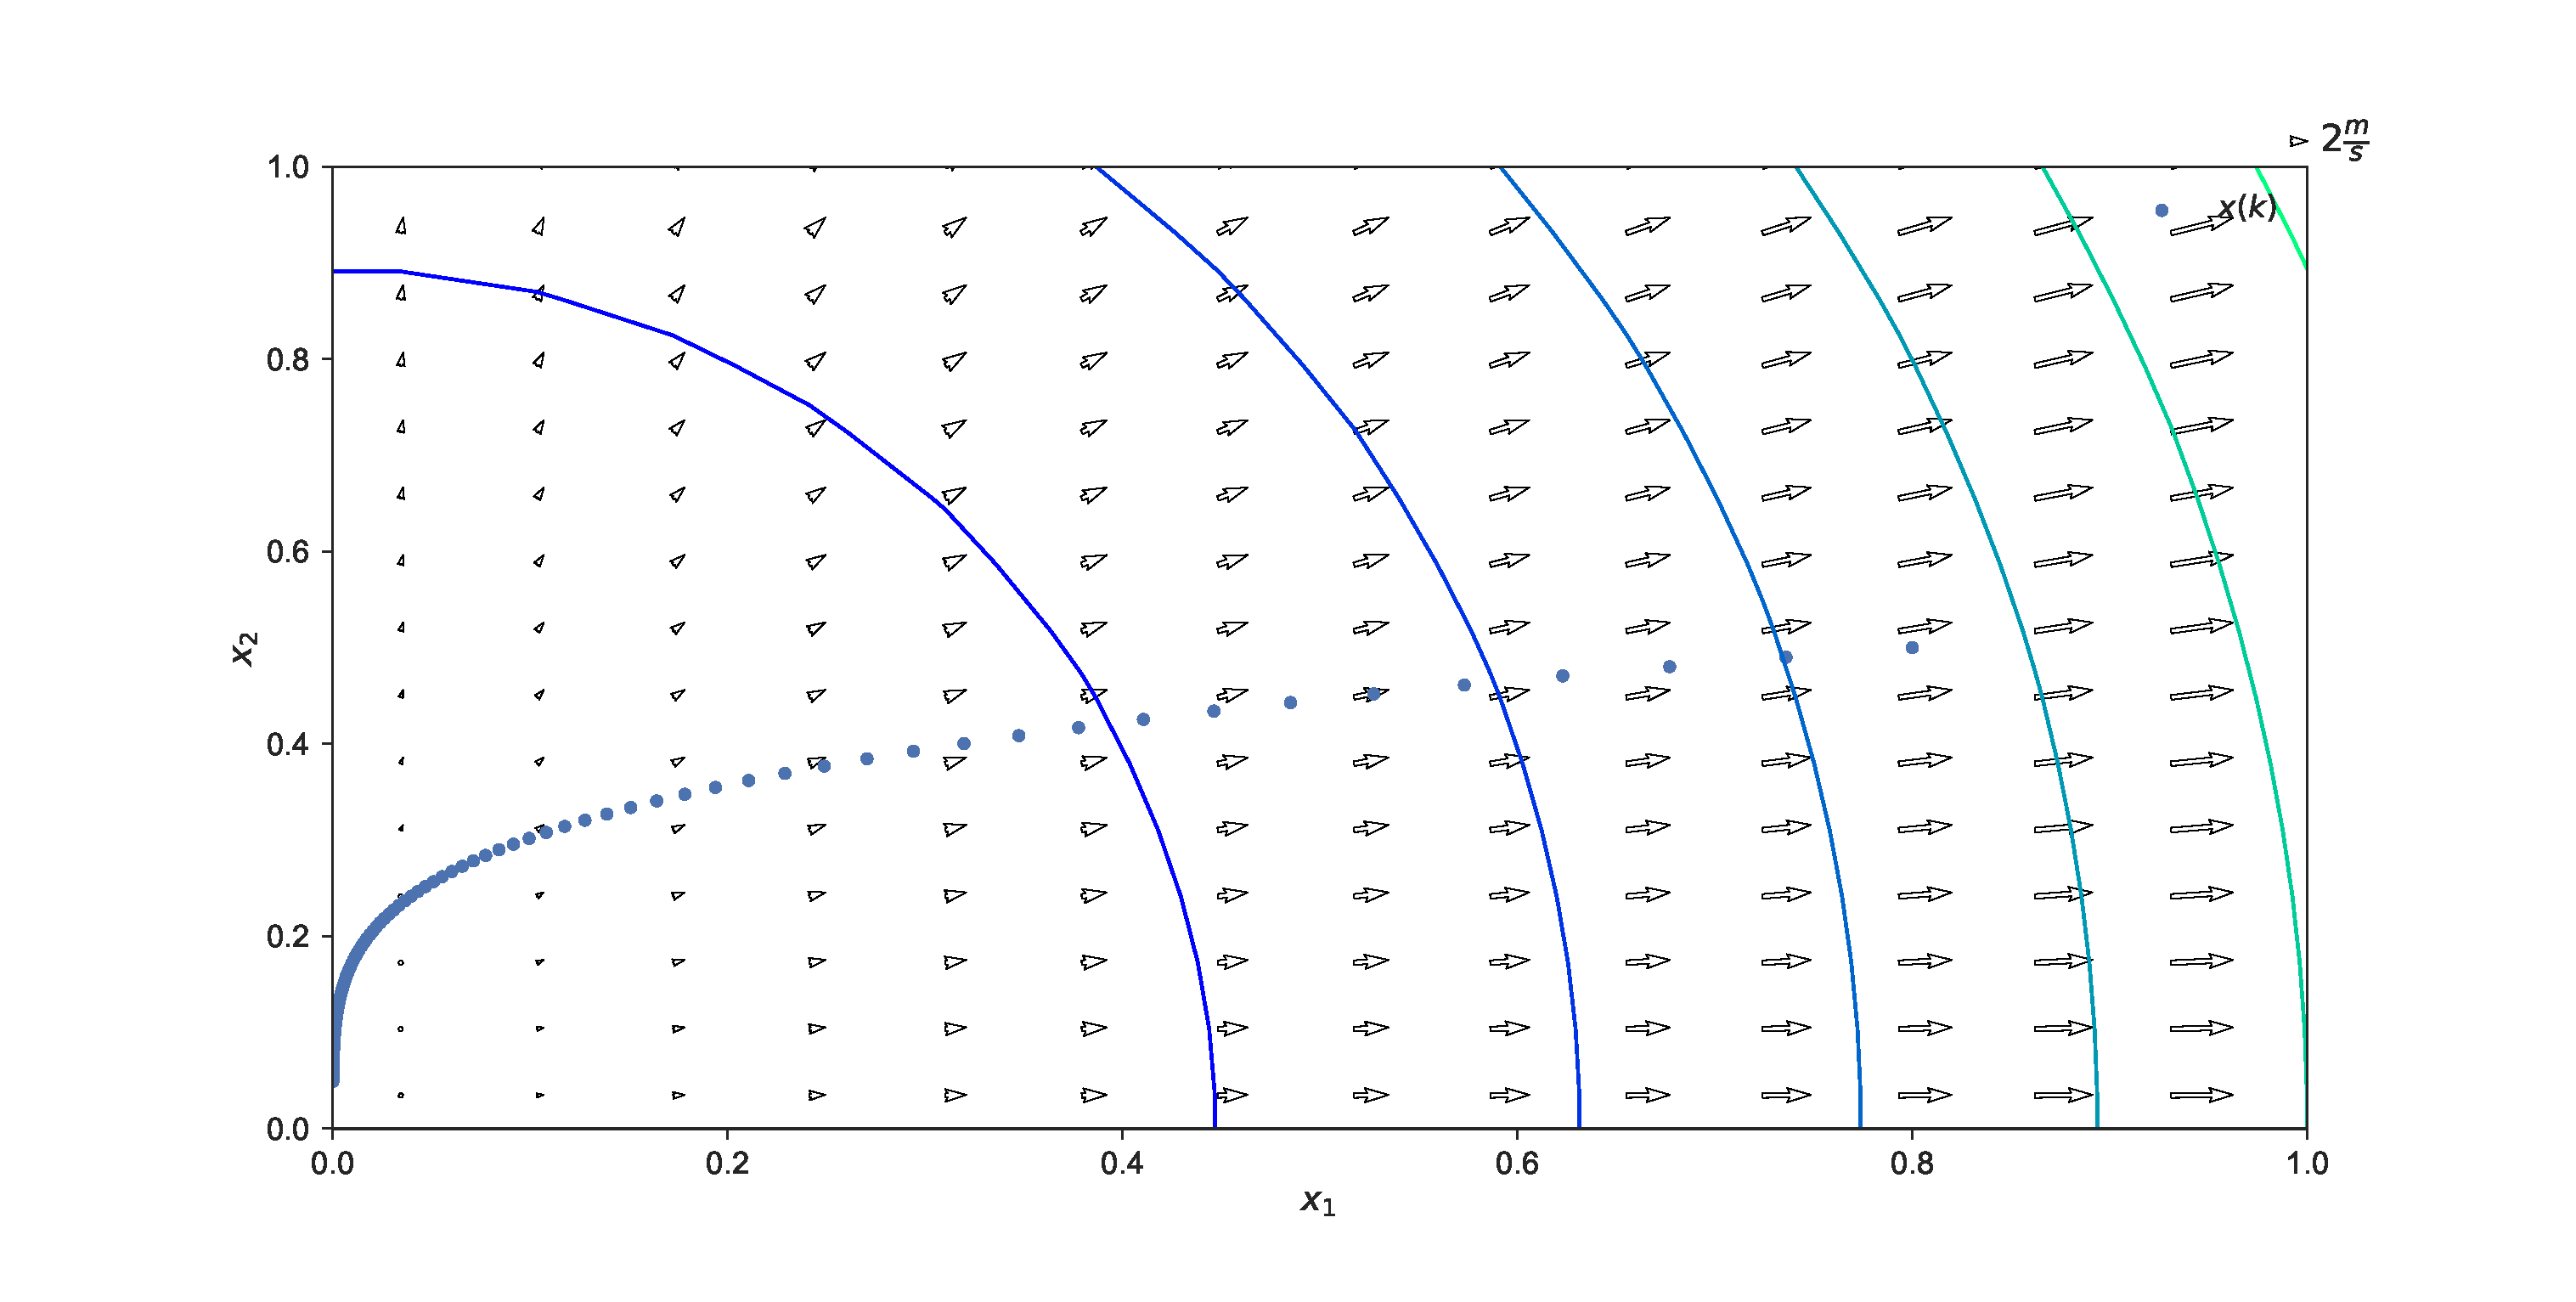
\includegraphics[width=\linewidth]{imgs/grad_contour.eps}
		\end{figure}
		\end{adjustwidth}
	}

	\subsection{Convergence Analysis}
	\frame[c]{
		\frametitle{Gradient Descent: Analysis}
		\begin{adjustwidth}{-2em}{-2em}
		Advantages:
		\begin{itemize}
			\item Every iteration is inexpensive

			\item Does not require second-order derivatives
		\end{itemize}

		Iterations:
		\begin{itemize}
			\item For every $k\in\mathbb{N}$, 
			\[f(x(k))-f(x^\ast)\leq \dfrac{1}{2k\alpha}||x^\ast-x(0)||_2\]

			\item The number of iterations such that $f(x(k))-f(x^\ast)<\varepsilon$
				  is $O(1/\varepsilon)$
		\end{itemize}
		\end{adjustwidth}
	}

	\frame[c]{
		\frametitle{Gradient Descent: Analysis (cont.)}
		% Src: http://www.seas.ucla.edu/~vandenbe/236C/lectures/gradient.pdf
		\begin{adjustwidth}{-2em}{-2em}
		Limit on convergence:
		\vspace{2em}
			\begin{tcolorbox}[title=Theorem (Nesterov)]
				For every integer $k\leq(n-1)/2$ and for every $x(0)\in D$,
				there exist functions satisfying the algorithms hypotheses 
				such that
				\[f(x(k)) - f(x^\ast)\geq \dfrac{3L||x^\ast-x(0)||_2^2}{32(k+1)^2}\]
			\end{tcolorbox}
		\end{adjustwidth}

	}


	\section[Method of Momentum]{Method of Momentum}
	\subsection{Formulation}
	\frame[c]{
		\frametitle{Tweaking the gradient descent}
		\underline{Todo:} make notation $x^+$ and $x(k+1)$ consistent
		Add a memory term to the gradient descent algorithm
		\begin{equation*}
			\left\{\begin{array}{rcl}
			z^+&=&\beta z+\nabla f(x)\\
			x^+&=&x-\alpha z^+\;,
			\end{array}
			\right.
		\end{equation*}
		\vspace{2em}
		where
		\[z^+:=z(k+1)\quad\text{and}\quad x^+:=x(k+1)\]
	}

	\frame[c]{
		\frametitle{Dynamics of momentum: Formulation (1/2)}
		\begin{adjustwidth}{-2em}{-2em}
		Let
		\[\begin{array}{rrcl}
		f:&\mathbb{R}^n&\to&\mathbb{R}\\
		&x&\mapsto&\dfrac{1}{2}x^\top Ax-b^\top x
		\end{array}
		\]
		where $A$ is symmetric, positive semi definite and nonsingular.

		\begin{equation*}
			\left\{\begin{array}{rcl}
			z^+&=&\beta z+(Ax-b)\\
			x^+&=&x-\alpha z^+\;.
			\end{array}
			\right.
		\end{equation*}
		\end{adjustwidth}

	}
	\frame[c]{
		\frametitle{Dynamics of momentum: Formulation (2/2)}
		
		Let $Q$ be such that $A=Q\Lambda Q^\top$.

		\begin{itemize} 
			\item Coordinate change
			\[w=Q(x-x^\ast)\quad\text{and}\quad y=Qz\]

			\item For each $i\in\mathbb{N}_{[1, n]}$,
			\begin{equation*}
			\left\{\begin{array}{rcl}
			y_i^+&=&\beta y_i+\lambda_i w_i\\
			w_i^+&=&-\alpha \beta y_i+(1-\alpha\lambda_i)w_i
			\end{array}
			\right.
		\end{equation*}
		This equation can be written as $v_i^+=R_iv_i$

		\item Let $v=(v_1,\ldots,v_n)$ and $R=\mathtt{blkdiag}(R_1,\ldots,R_n)$,
		\[v^+=Rv\]
		\end{itemize}
	}

	\frame[c]{
		\frametitle{Dynamics of momentum: Linear Difference Systems}
		\begin{adjustwidth}{-2em}{-2em}
			\begin{itemize}
			\item The convergence depends on the solutions to the system $v^+=Rv$;
			\vspace{3em}
			\item The analysis of the matrix $R$ provides the behaviour of the 
					convergence of the method;
			\vspace{3em}
			\item A solution to $v^+=Rv$, starting from an \emph{initial condition}
				$v_0$, is function $V:\mathbb{R}_{\geq0}\to\mathbb{R}^n$ defined as
				$V(k,v)$. 
			\end{itemize}
		\end{adjustwidth}
	}

	\frame[c]{
		\frametitle{Dynamics of momentum: Linear Difference Systems}
		\begin{adjustwidth}{-2em}{-2em}
		Equilibrium and stability
		\begin{itemize}
		\item The origin is an \emph{equilibrium point} to $v^+=Rv$ if $R\nu=0$

		\item  The origin is (Lyapunov) \emph{stable}
		if
		\[\forall\varepsilon>0, \forall v, \exists\delta>0:||v||_2<\delta\Rightarrow
		||V(k,0)||_2<\varepsilon, \forall k\in\mathbb{N}\]

		\item The origin is \emph{attractive} if
		\[\exists\delta>0, \forall ||v||_2<\delta, \lim_{k\to\infty} V(k,v)\to \nu\]

		\item The origin is \emph{asymptotically stable}
		if it is stable and attractive.
		\end{itemize}

		
		\end{adjustwidth}
	}

	\frame[c]{
		\frametitle{Dynamics of Momentum: Implications for $\alpha$ and $\beta$}
		\begin{itemize}
			\item Let $\sigma_1$ and $\sigma_2$ be the eigenvalues of $R$
		
			\item System $v^+=Rv$ is asymptotically stable if $\sigma_1$ and 
			$\sigma_2$ satisfy 
		\[\max\{||\sigma_1||_2, ||\sigma_2||_2\} <1\]

			\item Consequently, $\alpha$ and $\beta$ must satisfy the inequalities
		\[0<\alpha\lambda_i<2(1+\beta)\quad\text{and}\quad 0\leq\beta <1\]
		\end{itemize}
	}

	\frame[c]{
		\frametitle{Dynamics of Momentum: Types of Responses}
		\begin{adjustwidth}{-2em}{-2em}
		\begin{figure}[htpb!]
			\includegraphics[width=\linewidth]{imgs/2nd_order_responses.eps}
		\end{figure}
		\end{adjustwidth}
	}

	\frame[c]{
		\frametitle{Dynamics of Momentum: Example}
		\begin{adjustwidth}{-2em}{-2em}
		\[f(x,y)=4x^2+y^2\]
		\begin{figure}[htpb!]
			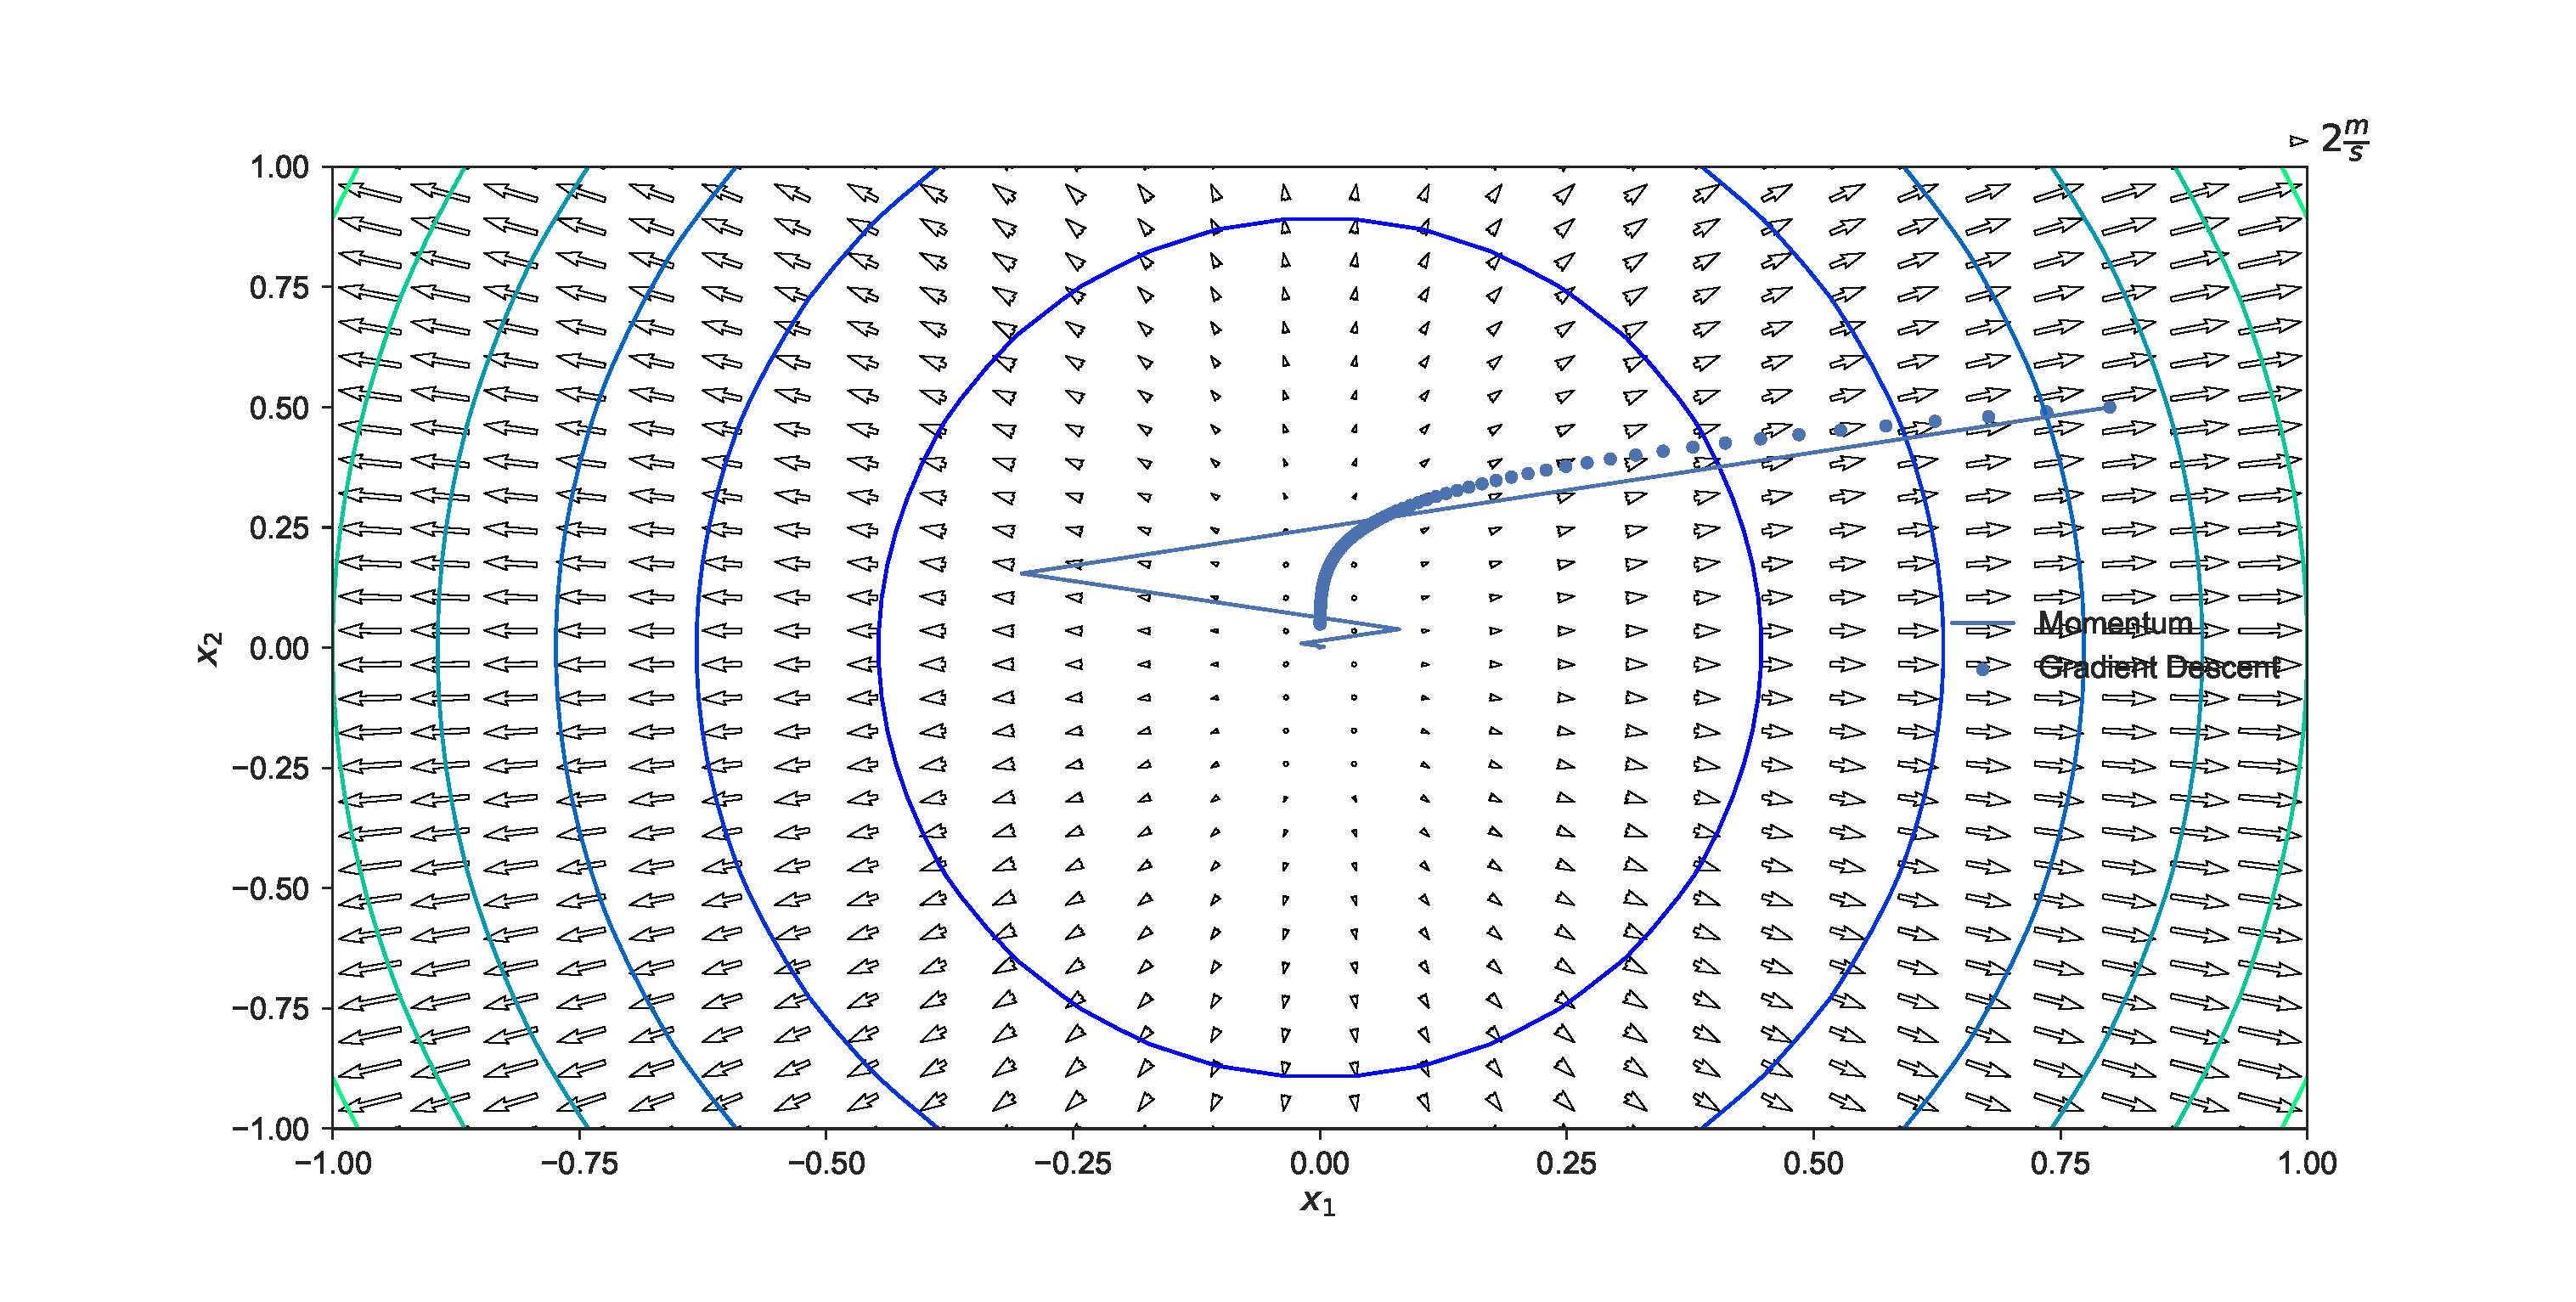
\includegraphics[width=\linewidth]{imgs/mom_contour.eps}
		\end{figure}
		\end{adjustwidth}
	}

	\frame[c]{
		\frametitle{Dynamics of Momentum: Comparison}
		\begin{adjustwidth}{-2em}{-2em}
		\begin{figure}[htpb!]
			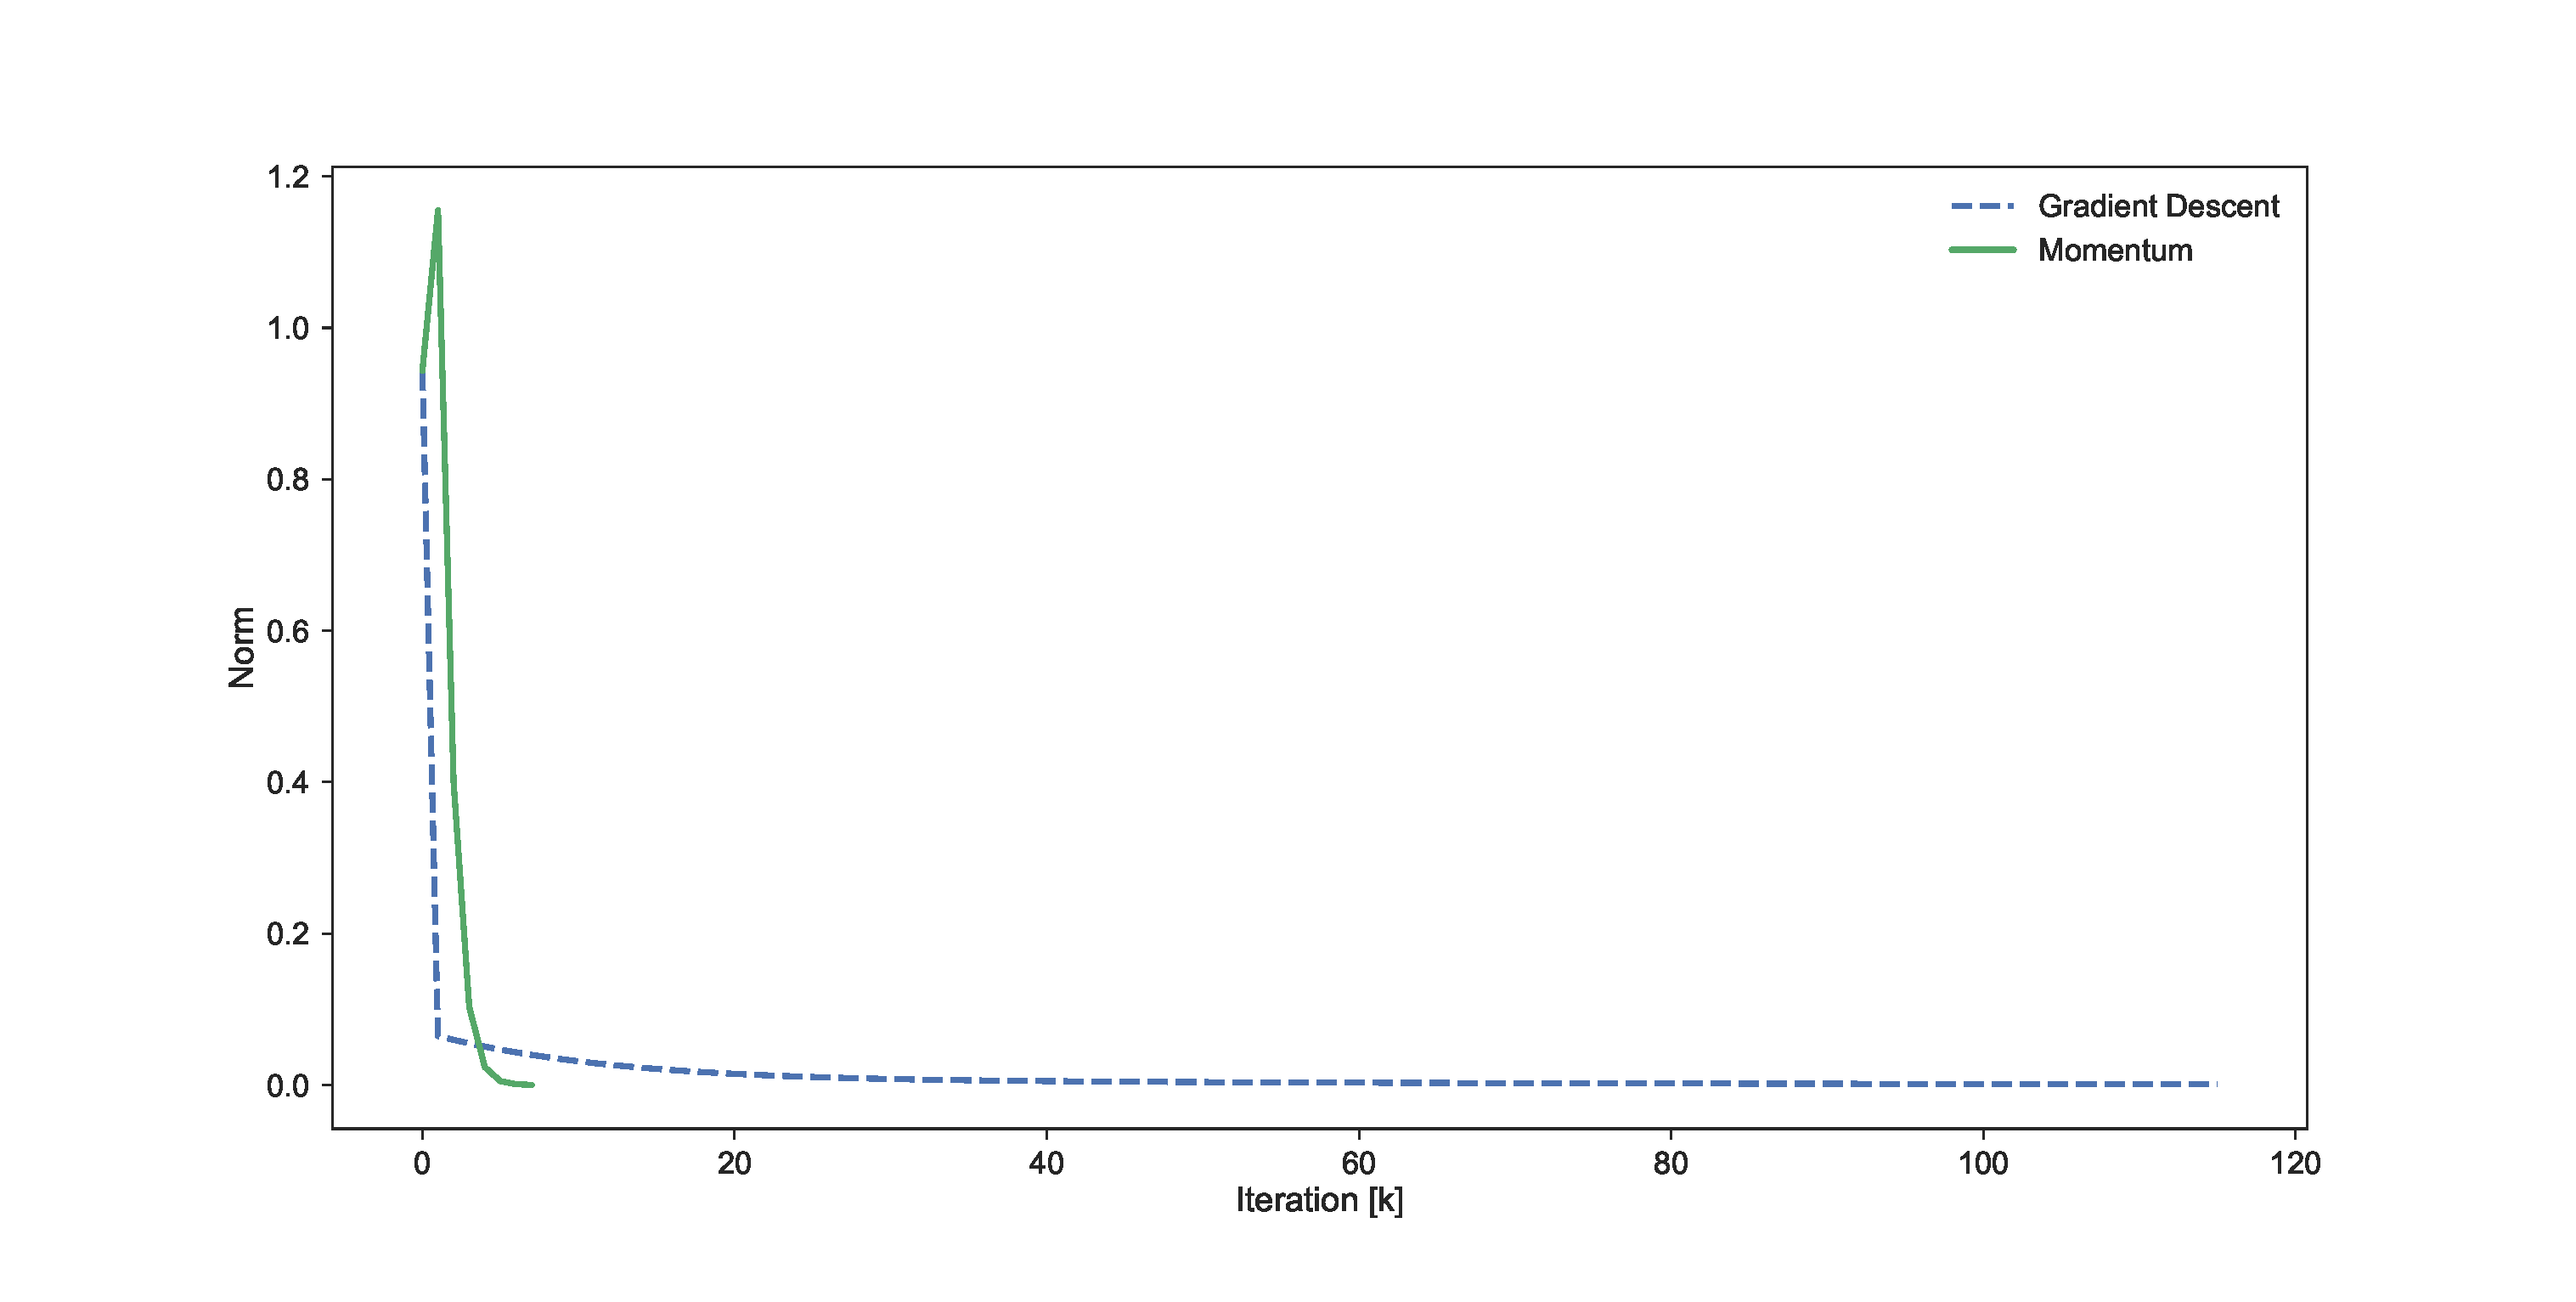
\includegraphics[width=\linewidth]{imgs/gd_mom_comp.eps}
		\end{figure}
		\end{adjustwidth}
	}

	\section{Conclusion}
	\subsection{Remarks}
	\frame[c]{
		\frametitle{Conclusion}
		\begin{itemize}
			\item We considered an unconstrained, convex problem modelled by class $\mathcal{C}^1$ functions 
			\vspace{2em}
			\item A method to find minimima over convex sets is using the gradient
			\vspace{2em}
			\item We consider method of momentum for the gradient descent
			\vspace{2em}
			\item Consists of adding a memory term to the gradient descent algorithm
		\end{itemize}
	}

	\subsection{Acknowledgment}
	\frame[c]{
		\frametitle{Thank you}
		References
		\begin{itemize}
			\item L. Vandenberghe, ``Optimization Methods for Large-Scale Systems''.
			\itshape{Lecture Notes}, UCLA
			\vspace{2em}
			\item S. Boyd, L. Vandenberghe, ``Convex Optimization''. \itshape{Cambridge University Press}, 2004.
		\end{itemize}
	}
		
\end{document}
